
\documentclass[xcolor=pdftex,dvipsnames,table,mathserif,aspectratio=169]{beamer}
\usetheme{default}
\usetheme{metropolis}
\usepackage{mathtools}
\setbeamersize{text margin left=.3in,text margin right=.3in} 

\DeclarePairedDelimiter\abs{\lvert}{\rvert}%
\DeclarePairedDelimiter\norm{\lVert}{\rVert}%


%\usetheme{Darmstadt}
%\usepackage{times}
%\usefonttheme{structurebold}

\usepackage[english]{babel}
%\usepackage[table]{xcolor}
\usepackage{pgf,pgfarrows,pgfnodes,pgfautomata,pgfheaps}
\usepackage{amsmath,amssymb,setspace,centernot}
\usepackage[latin1]{inputenc}
\usepackage[T1]{fontenc}
\usepackage{relsize}
\usepackage{pdfpages}
\usepackage[absolute,overlay]{textpos} 


\newenvironment{reference}[2]{% 
  \begin{textblock*}{\textwidth}(#1,#2) 
      \footnotesize\it\bgroup\color{red!50!black}}{\egroup\end{textblock*}} 

\DeclareMathSizes{10}{10}{6}{6} 

\begin{document}
\title{Part 8: Program Evaluation (f):\\
Synthetic Control Methods}
\author{Chris Conlon}
\institute{Applied Econometrics}
\date{\today}

\frame{\titlepage}
\begin{frame}{Motivation: Recap}
Difference in Difference approaches have some drawbacks:
\begin{itemize}
\item We need to really believe \alert{parallel trends}
\begin{itemize}
\item Is $\Delta PA$ really a good counterfactual for  $\Delta NJ$?
\item Obvious question: why not pick $\Delta DE$ or $\Delta NY$?
\item Measured effect shouldn't change if our assumption is valid (but it probably will!)
\end{itemize}
\item With multiple treated individuals we can use 2WFE estimator
\begin{align*}
y_{it} = \beta X_{it} + \delta_i \cdot T_{it} +  \gamma_i + \gamma_t + u_{it}
\end{align*}
\vspace{-0.8cm}
\begin{itemize}
\item It assumes \alert{additivity} of FE $\gamma_i + \gamma_t$ are independent!
\item States have different baseline levels $\gamma_i$ but evolution over time is common $\gamma_t$.
\item Turns out it doesn't really generalize the diff-in-diff with $I > 2$ (Imai and Kim 2020).
\end{itemize}            
\end{itemize}              
\end{frame}


\begin{frame}{Motivation: Recap}
Matching Estimators had drawbacks too:
\begin{itemize}
\item We need to believe in as if random-assignment conditional on $X$
\item CIA: $\{Y_i(1), Y_i(0)\} \perp T_i | X_i$.
\end{itemize}
But we could use pretty flexible methods in constructing our matched controls:           
\begin{itemize}
\item We could try to match on multiple dimensions of $X$.
\item $k\text{\textendash}NN$, kernels, etc.
\end{itemize}
What if we could use ideas from \alert{matching} to better satisfy something like our \alert{parallel trends} assumptions?
\end{frame}

\section{Example: Abadie, Diamond, Hainmueller (2010)}

\begin{frame}{The Question}
In 1988 California passes anti-smoking Prop 99
\begin{itemize}
\item increased excise tax by 25 cents per pack, 
\item earmarked the tax revenues to health and anti-smoking education budgets and funded anti-smoking ads
\item led to indoor smoking bans in restaurants and bars city by city
\end{itemize}
 What was the effect on per capita cigarette sales?
 \begin{itemize}
 \item Already a bunch of pre-existing trends.
 \item What is a good control for California?
 \end{itemize}
 Use state-level data from 1970-2000.
\end{frame}

\begin{frame}{The Idea}
Use a convex combination of other states to construct a \alert{synethetic counterfactual California}.\\
\begin{itemize}
\item We observe $Y_{it}, X_{it},T_{it}$.
\item Assume only $i=1$ and $t > T_0$ are \alert{treated}.
\item Construct a \alert{donor pool} of potential controls subscripted by $j$.
\item Choose some \alert{weights} $w_j$ for each entity (state) in donor pool. How?
\begin{itemize}
\item Same $\mathbf{X_{1}} = \sum_j w_j \mathbf{X_{j}}$ as treated observations (like matching).
\item Same $\left({Y_{1,1},\ldots, Y_{1,T_0}} \right)= \sum_j w_j \cdot \left({Y_{j,1},\ldots, Y_{j,T_0}} \right)$ (like parallel trends).
\item Weights sum to one $\sum_j w_j = 1$ and maybe are non-negative (or not!)
\end{itemize}
\item Idea is to match all of the $X$'s and all of the $Y_{it}$'s in the \alert{pre-period}
\end{itemize}
\end{frame}

\begin{frame}{Covariate Balance}
\begin{center}
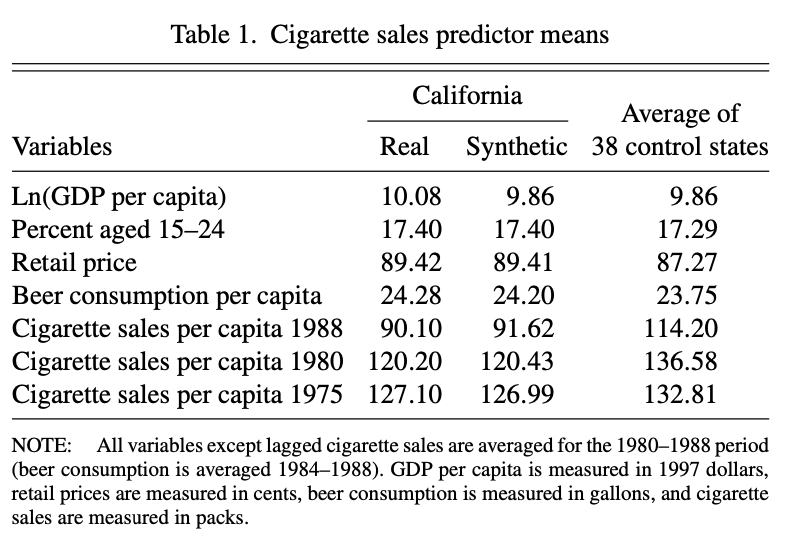
\includegraphics[width=4.5in]{./resources/abadie_1.png}
\end{center}
\end{frame}

\begin{frame}{Donor Weights}
\begin{center}
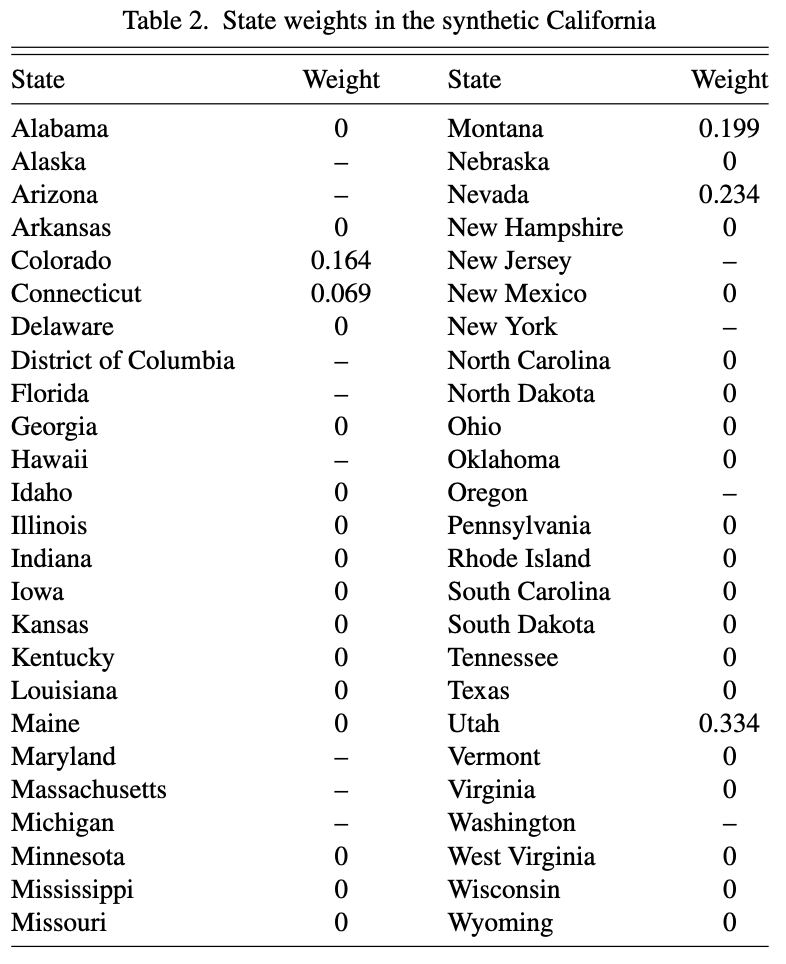
\includegraphics[width=2.5in]{./resources/abadie_2.png}
\end{center}
\end{frame}

\begin{frame}{Trend Check and Treatment Effects}
\begin{center}
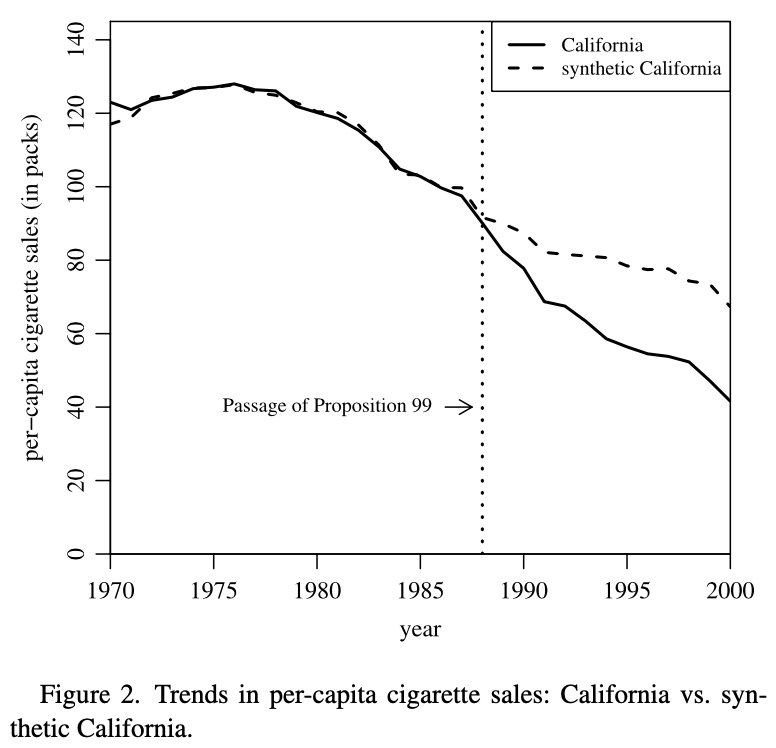
\includegraphics[width=2.75in]{./resources/abadie_3.png}
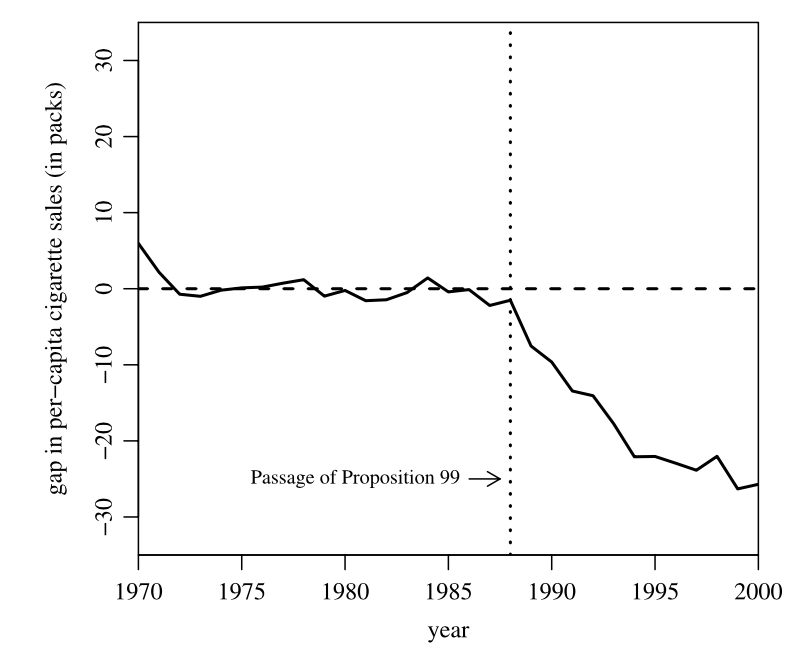
\includegraphics[width=2.75in]{./resources/abadie_4.png}
\end{center}
\end{frame}

\begin{frame}{But still some issues}
\begin{itemize}
\item How sensitive are weights estimates to different covariates?
\begin{itemize}
\item ``state-level measures of unemployment, income inequality, poverty, welfare transfers, crime rates, drug related arrest rates, cigarette taxes, population density, and numerous variables to capture the demographic, racial, and social structure of states''.
\end{itemize}
\item Can we run a \alert{placebo check}? Do we detect effects where we know there is a null effect?
\begin{itemize}
\item Put California in the donor pool.
\item Pick a state from the donor pool at pretend that receives the treatment after $T_0$
\item Choose $w_j$ following the synthetic control procedure.
\item Compute the treatment effects in the same way.
\item Repeat for all states in donor pool.
\item Compare \alert{mean-square prediction error} (MSPE) for $(Y_{1,1},\ldots,Y_{1,T_0})$
\item This doubles as \alert{inference}.
\end{itemize}
\end{itemize}
\end{frame}



\begin{frame}{Placebo Test}
\begin{center}
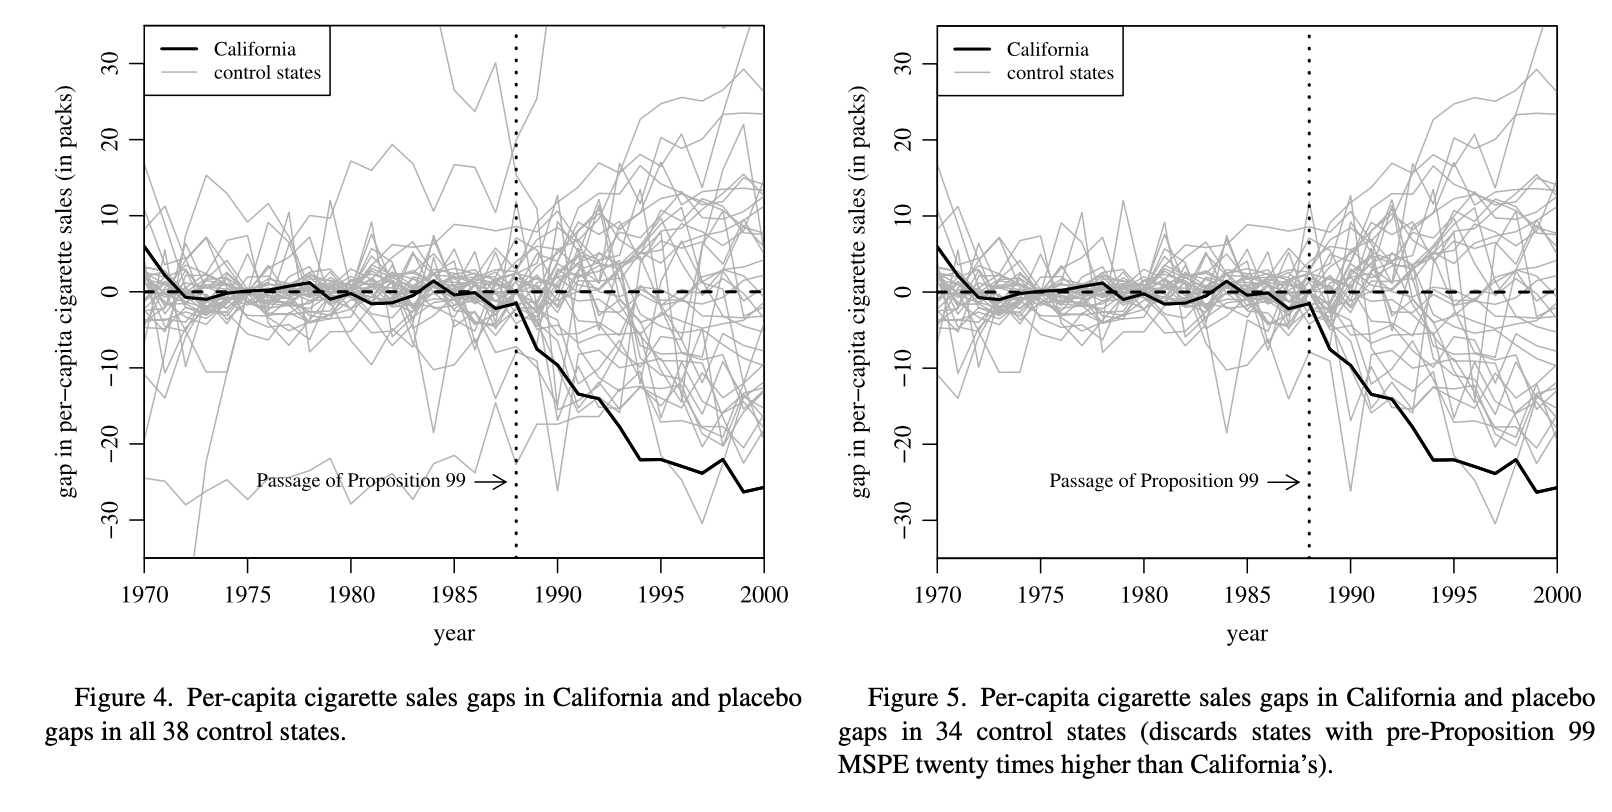
\includegraphics[width=5in]{./resources/abadie_5.png}
\end{center}
\end{frame}


\begin{frame}{More Placebo Tests: How unusual is the CA result?}
\begin{center}
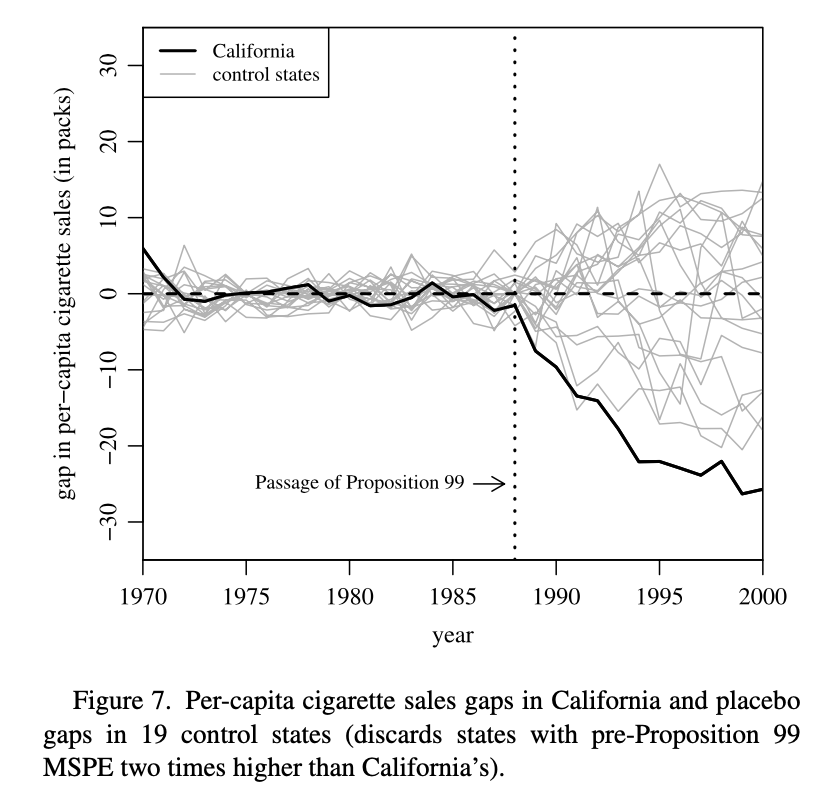
\includegraphics[width=2.75in]{./resources/abadie_6.png}
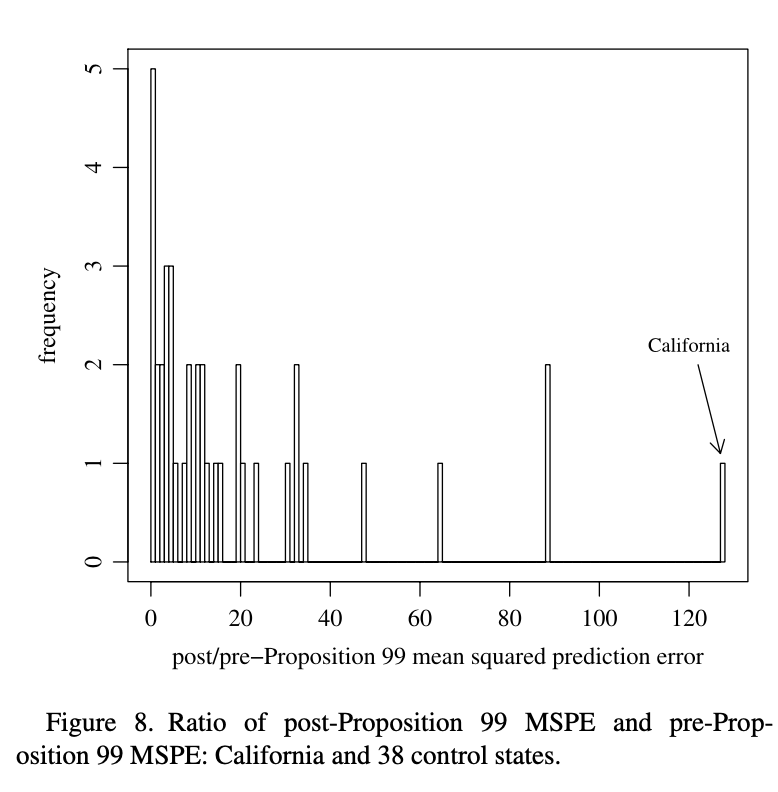
\includegraphics[width=2.75in]{./resources/abadie_7.png}
\end{center}
\end{frame}


\begin{frame}{More Formally}
We're going to break this down into three parts:
\begin{enumerate}
\item How do we estimate $w_j$?
\item Conditional on $\hat{w}_j$'s, how do we estimate the treatment effect?
\item What kinds of models are compatible?
\end{enumerate}
\end{frame}


\begin{frame}{A Starting Point}
Start with $T_{it} =1$ IFF $i =1$ and $t > T_0$:
\begin{align*}
Y_{it} = Y_{it}(0)  + \alpha_{it} T_{it}
\end{align*}
Estimate $\mathbf{\boldsymbol{\alpha}_1} =(\alpha_{1, T_0+1},\alpha_{1, T_0+2},\ldots,\alpha_{1,T}) $ (period by period treatment effect).\\
 For $t > T_0$:
\begin{align*}
\alpha_{1 t}=Y_{1 t}(1)-Y_{1 t}(0)=\underbrace{Y_{1 t}}_{\text{observed}}-\underbrace{Y_{1 t}(0)}_{\text{counterfactual}}
\end{align*}

\end{frame}

\begin{frame}{A Starting Point}
Consider the model
\begin{align*}
Y_{i t}(0)=\gamma_{t}+ \theta_{t} \mathbf{Z}_{i}+\lambda_{t} \mathbf{F}_{i}+u_{i t}
\end{align*}
\begin{itemize}
\item $\delta_t$ is the time fixed effect
\item $Z_i$ are the usual covariates (fixed in $i$ over time) with potentially time varying coefficients.
\item $F_i$ are $i$ specific \alert{unobserved factors}. Estimating these are complicated.
\item $\lambda_t$ are called \alert{factor loadings}.
\end{itemize}
This is a generalization of the usual additive $\gamma_t + \gamma_i$ fixed effects model called \alert{interactive fixed effects} (Bai 2009).
\end{frame}

\begin{frame}{Some Algebra}
So we define the synthetic observation as:
\begin{align*}
\sum_{j=2}^{J+1} w_{j} \underbrace{Y_{j t}(0)}_{\text{observed}}=\delta_{t}+\boldsymbol{\theta}_{t}\left(\sum_{j=2}^{J+1} w_{j} \mathbf{Z}_{j}\right)+\lambda_{t}\left(\sum_{j=2}^{J+1} w_{j} \boldsymbol{F}_{j}\right)+\sum_{j=2}^{J+1} w_{j} u_{j t}
\end{align*}
And the difference in untreated observations:
\begin{align*}
\begin{aligned}
Y_{1 t}(0)-\sum_{j=2}^{J+1} w_{j} Y_{j t}(0)\\
=\boldsymbol{\theta}_{t} \underbrace{\left( \mathbf{Z}_{1}-\sum_{j=2}^{J+1} w_{j} \mathbf{Z}_{j} \right)}_{\text{ match this directly}} 
&+\lambda_{t} \underbrace{\left(\boldsymbol{F}_{1}-\sum_{j=2}^{J+1} w_{j} \boldsymbol{F}_{j}\right)}_{\text{match indirectly:  }  (Y_{i,1},\ldots,Y_{i,T_0})}+\sum_{j=2}^{J+1} w_{j}\underbrace{\left(u_{1 t}-u_{j t}\right)}_{\text{Usual} E[u_{it} | \mathbf{Z}_{it}, \mathbf{F}_{it} ]=0}
\end{aligned}
\end{align*}
\end{frame}


\begin{frame}{Some Algebra}
The goal is to match:
\begin{align*}
\mathbf{Z}_{1}= \sum_{j=2}^{J+1} w_{j} \mathbf{Z}_{j}, \quad
\mathbf{F}_{1} \approx \sum_{j=2}^{J+1} w_{j} \mathbf{F}_{j} 
\end{align*}
\begin{itemize}
\item The main result in the Abadie et. al (2010) paper proves that the above equation holds approximately if 
$$\left({Y_{1,1},\ldots, Y_{1,T_0}} \right)= \sum_j w_j \cdot \left({Y_{j,1},\ldots, Y_{j,T_0}} \right)$$
\item This frame generalizes the 2WFE model since we can use time dimension to difference them out.
\item We cannot difference out the $\lambda_t \mathbf{F}_i$.
\end{itemize}
\end{frame}


\begin{frame}{The Challenge}
Theory depends on matching:
\begin{align*}
\mathbf{Z}_{1}= \sum_{j=2}^{J+1} w_{j} \mathbf{Z}_{j}, \quad
\left({Y_{1,1},\ldots, Y_{1,T_0}} \right)= \sum_j w_j \cdot \left({Y_{j,1},\ldots, Y_{j,T_0}} \right)
\end{align*}
\begin{itemize}
\item One problem is the \alert{convex hull} problem. 
\begin{itemize}
\item There may be no $w_2,\ldots,w_J$ that satisfy the equations 
\end{itemize}
\item Instead choose $\mathbf{w}$ in a \alert{minimum distance sense} with some weighting matrix $\Omega$
\begin{itemize}
\item Can choose $\Omega$ to minimize variance of the resulting estimator.
\end{itemize}
\item Hard to fit crazy out of bounds values: can't match $CA$ population as linear combination of other states!
\end{itemize}
\end{frame}

\begin{frame}{Other Pitfalls}
Other things can go wrong
\begin{align*}
\mathbf{X}_{i}&=\left(\mathbf{Z}_{i}, Y_{i,1},\ldots, Y_{i,T_0} \right)\\
\arg \min_{w_2,\ldots, w_J}&  (\mathbf{X}_{i}-\sum_j w_j \mathbf{X}_{j})' \Omega  (\mathbf{X}_{i}-\sum_j w_j \mathbf{X}_{j}) \quad \text{ s.t. }  \sum_j w_j =1
\end{align*}

\begin{itemize}
\item Can get negative weights: what do those mean? 
\item We can rule them out $w_j \geq 0$ constraints but the problem becomes more difficult to solve.
\item This starts to look like a familiar LASSO problem: quadratic objective, $L_1$ penalty!
\item We shouldn't be surprised by sparse models.
\end{itemize}
\end{frame}

\begin{frame}{In practice}
\begin{itemize}
\item The R package \texttt{synth} and accompanying examples are a good start.
\item The R package \texttt{MSCMT} fixes some of the optimization issues in \texttt{synth}.
\begin{itemize}
\item When there is no set of feasible weights and the non-negativity constraint binds -- the problem is tricky to solve
\item \texttt{synth} can produce sub-optimal solutions (and slowly).
\end{itemize}

\end{itemize}

\end{frame}


\begin{frame}{A more unified view}
We can ask -- what are the implied regression weights for linear regression? What is $E[Y_{1,t}(0) | \mathbf{X}]$?
\begin{itemize}
\item Get coefficients using just donor pool: $\widehat{\boldsymbol{B}}=\left(\overline{\boldsymbol{X}}_{0} \overline{\boldsymbol{X}}_{0}^{\prime}\right)^{-1} \overline{\boldsymbol{X}}_{0} \boldsymbol{Y}_{0}^{\prime}$
\item Predict $Y_{1,t}(0) = \widehat{\boldsymbol{B}}^{\prime} \overline{\boldsymbol{X}}_{1}$.
\item Same as synthetic control but with weights: $\boldsymbol{W}^{r e g}=\overline{\boldsymbol{X}}_{0}^{\prime}\left(\overline{\boldsymbol{X}}_{0} \overline{\boldsymbol{X}}_{0}^{\prime}\right)^{-1} \overline{\boldsymbol{X}}_{1}$ (Projection matrix).
\end{itemize}
Why? Remember, \alert{everything is a kernel} our prediction of $E[Y | X]$ is always some weighted average of other $Y_j$'s.
\end{frame}

\begin{frame}{Additonal Applications}
\begin{itemize}
\item What is word of mouth effect of Superbowl ads? (Lovett, Peres, Xu QME 2019)
\begin{itemize}
\item Construct synthetic versions of brands that don't buy Superbowl ads
\end{itemize}
\item What is effect of soda tax on consumption in Berkeley, CA ? (Bollinger Sexton WP 2019).
\begin{itemize}
\item Construct synthetic drugstores, supermarkets, and convenience stores using two donor polls: inside CA and outside CA.
\end{itemize}
\item What are economic effects of German reunification?
\begin{itemize}
\item Now we need a counterfactual ``West Germany'' (!) \\
(Abadie, Diamond, and Hainmueller 2015)
\end{itemize}
\end{itemize}
\end{frame}

\begin{frame}{Weighting}
\begin{center}
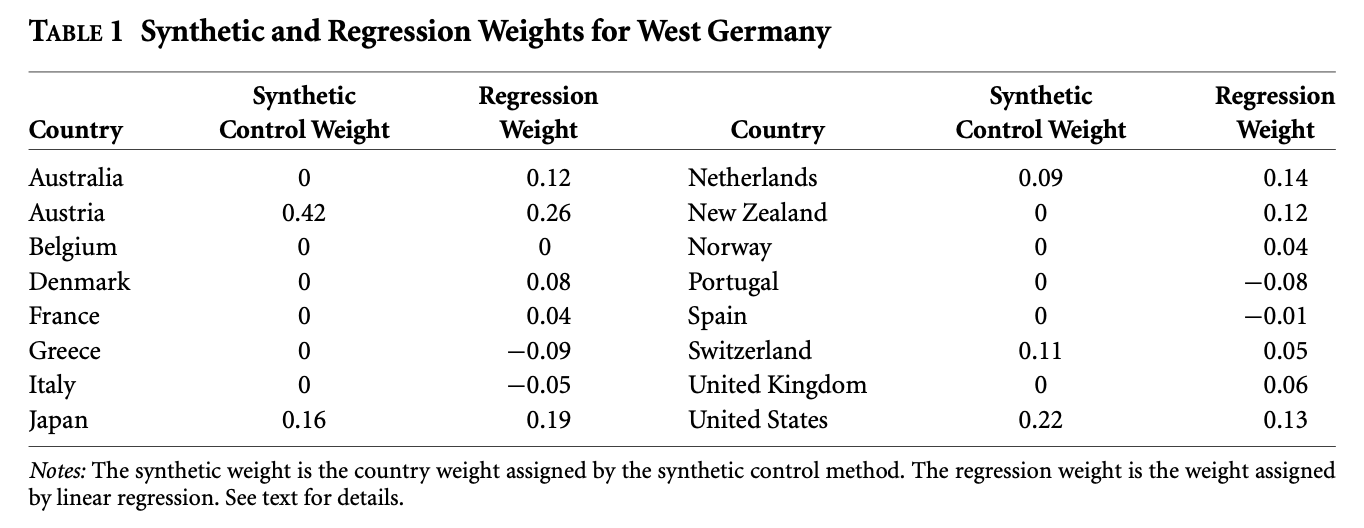
\includegraphics[width=6in]{./resources/germany_1.png}
\end{center}
\end{frame}

\begin{frame}{Balance Table}
\begin{center}
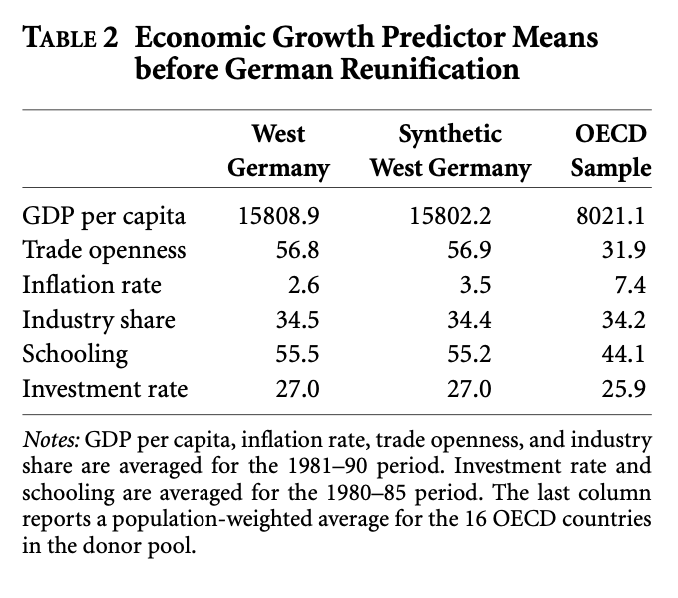
\includegraphics[width=3.2in]{./resources/germany_2.png}
\end{center}
\end{frame}

\begin{frame}{Treatment Effects}
\begin{center}
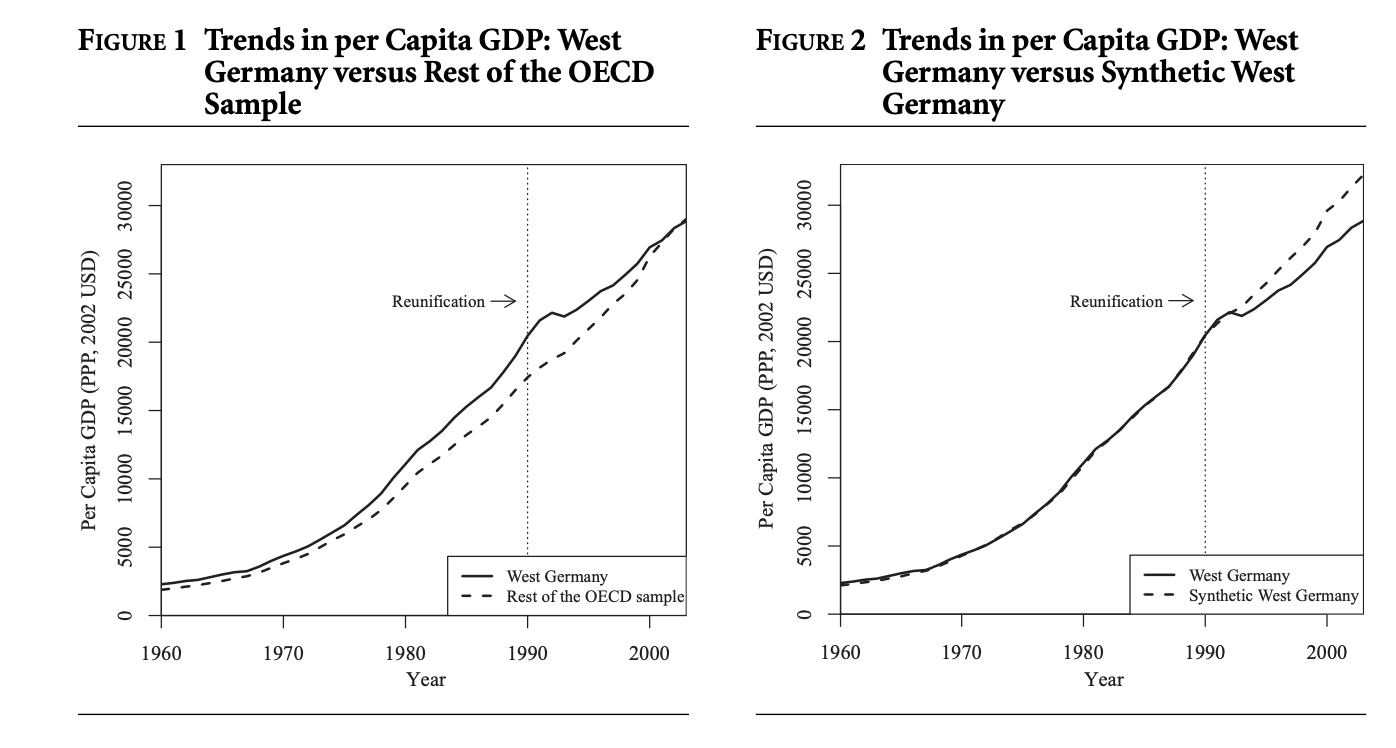
\includegraphics[width=5.5in]{./resources/germany_3.png}
\end{center}
\end{frame}


\begin{frame}{Treatment Effects and Placebo Timing}
\begin{center}
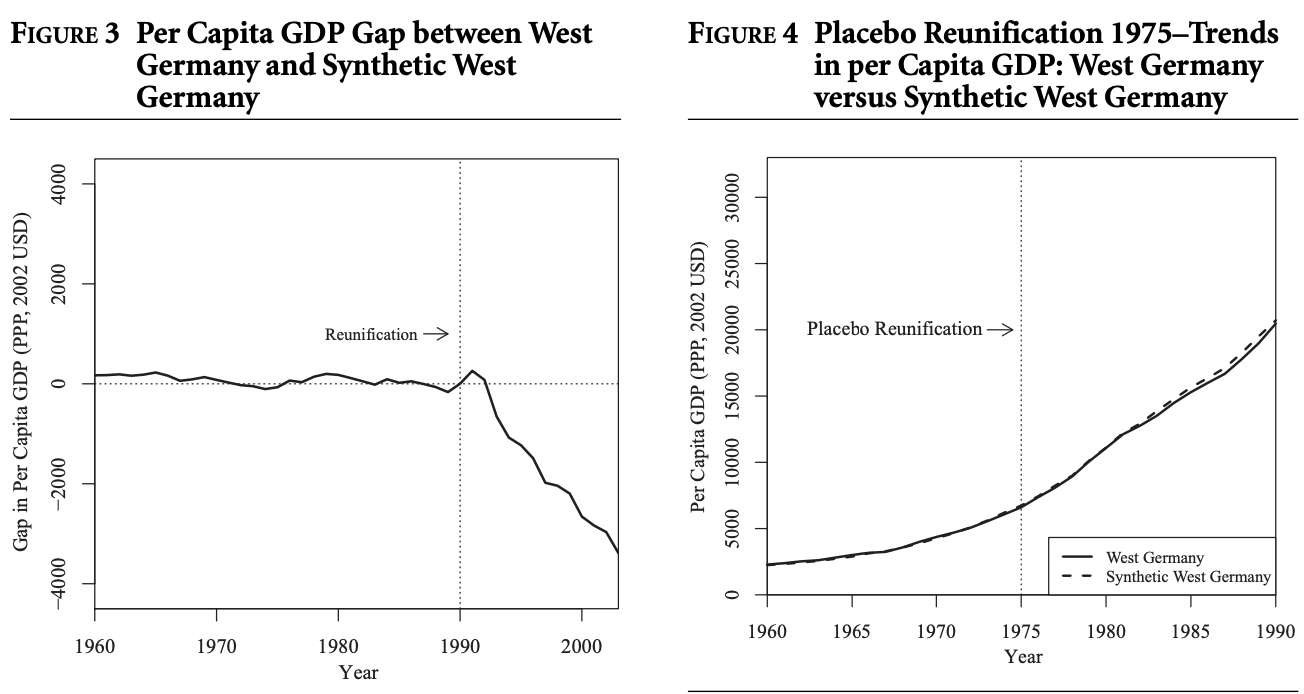
\includegraphics[width=5.5in]{./resources/germany_4.png}
\end{center}
\end{frame}

\begin{frame}{Treatment Effects and Placebo Timing}
\begin{center}
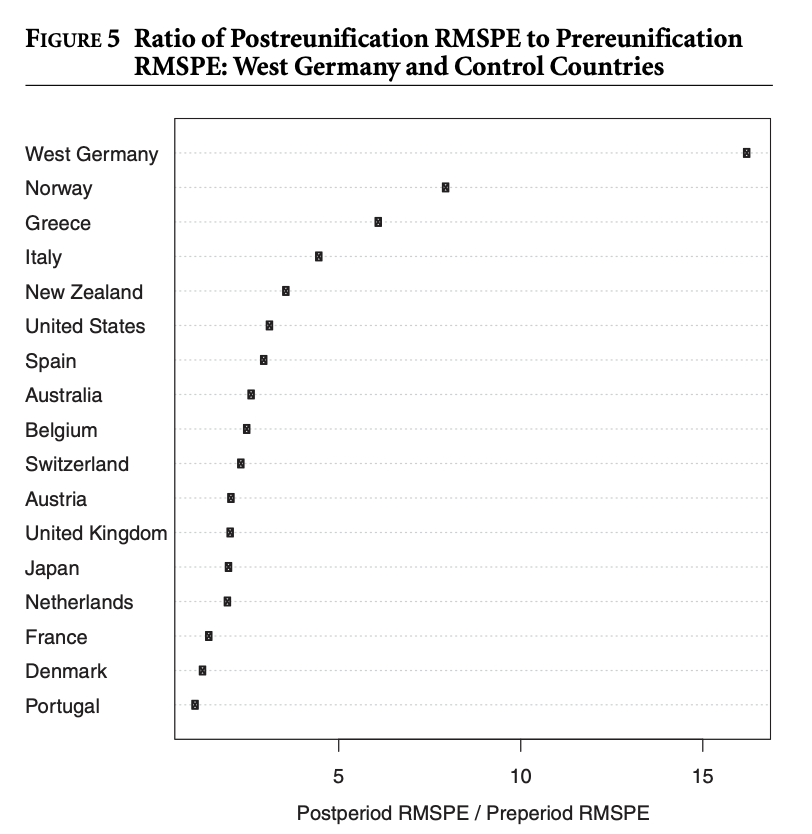
\includegraphics[width=2.8in]{./resources/germany_5.png}
\end{center}
\end{frame}

\section{Thanks}



\end{document}
\item (for now) only first unit $i=1$ gets treated after $T_0$.
$T_{it}= \begin{cases}
1 & \text{ if } i=1, t \geq T_0 \\
0 & \text{ o.w.}
\end{cases}
$

